
\begin{frame}
\frametitle{Contributions}
\begin{itemize}
  \item \emph{Selectively} using prior, similarity (entity - mention) and coherence (entity - entity) 
  depending on the text\bigskip
  \item Keyphrase based mention - entity similarity\bigskip
  \item Modeling of the problem \bigskip
\end{itemize}
\end{frame}

\begin{frame}
 \frametitle{Mention Entity Graph}
 \begin{figure}[h]
 \centering
 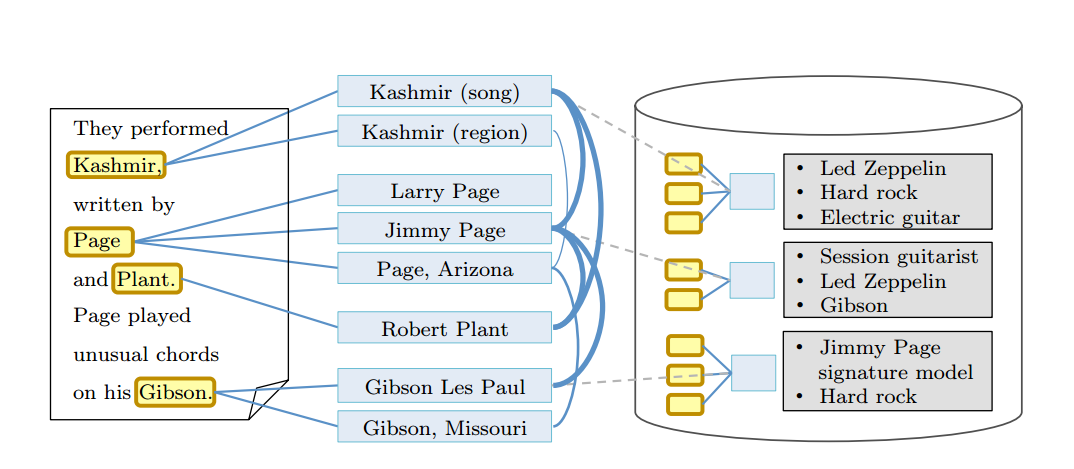
\includegraphics[bb=0 0 1074 469,scale=0.3]{./megraph.png}
 % megraph.png: 1074x469 pixel, 72dpi, 37.88x16.54 cm, bb=0 0 1074 469
 \caption{Mention Entity Graph}
\end{figure}


\end{frame}

\begin{frame}
 \frametitle{Recognition and Selecting Candidate Entities : Nodes of the graph}

 \begin{itemize}
  \item  Stanford's NER is used for finding potential named entity \medskip
  \item Yago provides short names and paraphrases for each entity via the ``means'' relation \medskip
  \item The list can be huge. Eg., For Afghanistan \medskip
 \begin{itemize}
 
 \item  Dari Persian 
 \item Third Anglo Afghan War 
\item  Republic of Afghanistan 
 \item Afghanistan at the Asian Games 
\end{itemize}
\end{itemize}
\end{frame}

\begin{frame}{Keyphrase based similarity : Edge weights}
\begin{itemize}  
\item Keyphrases for entities
  \begin{itemize}
    \item Link anchor text
    \item Category Names, citation titles, external references
    \item Titles of articles linking to the entity
  \end{itemize}
\item \textbf{How important is each word?}
\item $ weight(w) = \frac{|w \in (KP(e)_{e'\in IN_e}KP(e'))|}{N} $
Here, $IN$ refers to the set of entities that have in links to $e$
\item Higher the weight, more indicative is a word of the topic. Statistics will have a higher weight for Prof. Michael Jordan.
\end{itemize}
\end{frame}

\begin{frame}
 \frametitle{Keyphrase based similarity}
 Given a mention, m, we have all the candidate entities ($E$) with their respective keyphrase sets.
 We need to find sim(m, e) for all $e \in E$
 \begin{itemize}  
  \item For a given entity, for each keyphrase, find its \emph{cover}.  \medskip
  \item \emph{Cover} : Shortest window of words that contains maximal number of words of the keyphrase. \medskip
  \item Keyphrase : ``Grammy Award Winner'' \medskip
  \item ``He has been the  \textcolor{green}{winner of many awards during his long career including the Grammy}''  \medskip
\end{itemize} 
\end{frame}


\begin{frame}
 \frametitle{Keyphrase based similarity : Scoring}
  \begin{center}
  $score(q) = z * \frac{\Sigma_{w \in cover} weight(w)}{\Sigma_{w \in q} weight(w)}$\\ \bigskip
  q : Partially matching phrase
  $simscore(m, e) = \Sigma_{q \in KP(e)} score(q)$
  \end{center}
  For entity - entity similarity, Milne-Witten similarity measure was used.
 \end{frame}

\begin{frame}
\frametitle{Robustness : Selectively picking prior, similarity and concreteness}
\begin{itemize}
 \item Use prior only if prior for some candidate is above 90\% \bigskip
 \item Invoke coherence only if there is \emph{scope} for coherence to improve something \bigskip
 \item $diff = \Sigma_{i=1...k}|prior(m, e_i) - simscore(m, e_i)|$ \bigskip
 \item If diff is not \textgreater  0.9, choose the best candidate entity using only prior and simscore \bigskip
\end{itemize}
\end{frame}